\documentclass{article}
 \usepackage{graphicx}
 


\title{HW1 Getting Started}
\author{Fei Ding}

\begin{document}
\maketitle

Problem 1

I obtained $gfortran$ from http://www.macresearch.org/gfortran-leopard, and $gcc$ from http://hpc.sourceforge.net/. 

But I came up to a problem as following: 

gfortran: error trying to exec 'as': execvp: No such file or directory. 

I think this is because the $gcc$ and $gfortran$ were not in the same path, I tried to path $gcc$, but I could not path it without super user's password.  I tried the only password I knew for my mac, but it failed.


I would try to figure out these things as soon as possible but now I would like to submit this in time.
 
\vskip 1cm




Problem 2
\begin{figure} [ht]
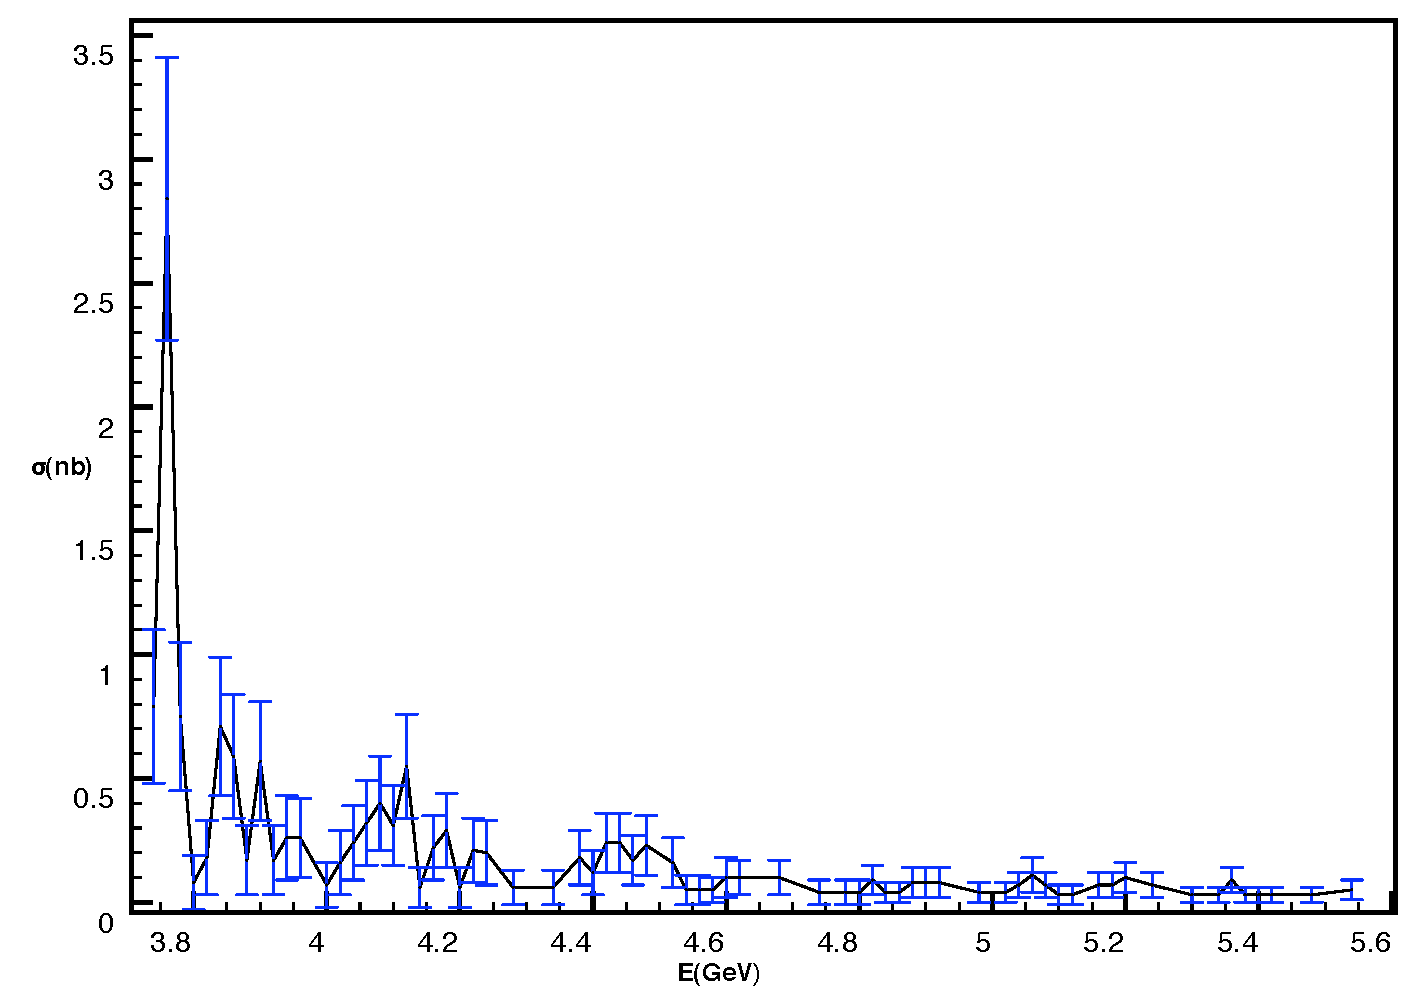
\includegraphics[width=1.0\textwidth]{hw1}
\end{figure}

I obtained the program $Plot$ from http://www.apple.com/downloads/macosx/math\_science/plot.html.  The program was automatically installed after the zip file was fully downloaded.  I produced a pdf version of the figure.

However, I would try to switch to gnuplot later.

\vskip 1cm



Problem 3
 \begin{displaymath}
 \int^\infty_0\Pi_{\mu\nu}\left(\vec{r}\right)\,d^3r=\frac{F_{\mu\nu}}{\pi}\cite{Oetiker}
 \end{displaymath}
 
 I obtained the distribution $MacTex$ from http://www.tug.org/mactex/.  I double clicked the MacTex-2008.mpkg and it was automatically installed.
 
 \vskip4cm
 \begin{thebibliography}{99}
 \bibitem{Oetiker}
 The Not So Short Introduction to LaTex2e, by Tobias Oetiker, Hubert Partl, Irene Hyna and Elisabeth Schlegl.
 \end{thebibliography}
 
 \end{document}